\documentclass[a4paper,11pt,titlepage]{article}

\usepackage{latexsym}
\usepackage{graphicx}
\usepackage{float}
\usepackage{url}
\usepackage{unicode}
\usepackage[polish]{babel}
\usepackage{titlesec}

\newcommand{\sectionbreak}{\clearpage}
\author{Adam Talarczyk}
\title{Projektowanie aplikacji mobilnych}
\frenchspacing
\begin{document}
\begin{titlepage}
    \begin{center}
        \vspace*{1cm}
 
        \Huge
        \textbf{Projektowanie webowych aplikacji graficznych}
 
        \vspace{0.5cm}
        \LARGE
        ``One-armed bandit''


Gra przeglądarkowa
 
        \vspace{1.5cm}
 
        \textbf{Adam Talarczyk}
 
        \vfill
 
        \vspace{0.8cm}
 
        \Large
        Wydział Nauk Ścisłych i Technicznych

        Uniwersytet Śląski

	Semestr letni 2020/2020
 
    \end{center}
\end{titlepage}
\newpage
\tableofcontents
\newpage

\section{Wstęp}
\subsection{Założenia projektowe}
Projekt ma na celu realizację``jednorękiego bandyty'' (inaczej zwanego maszyną wrzutową) - automatu hazardowego, który dobiera losowe konfiguracje symboli. Podział automatów ze względu na tryb gry jest wiele, można je kategoryzować pod względem ilości walców i możliwości kombinacji wygranej. Projekt skupia się na wariancie 3-walcowym, gdzie jedyną możliwością wygranej jest jedna, pozioma linia z trzema takimi samymi symbolami.

Gracz na samym początku dysponuje określoną ilością gotówki, za którą może zakręcić kołem. Wirtualne nagrody mieszczą w zakresie od \verb|$10| do \verb|$200000| i zależą stawki, jaką ustawi gracz. Stawka może być wybrana od \verb|$50| do \verb|$1000|. Każde \verb|$50| więcej, to dodatkowy mnożnik, zatem grając z najwyższą stawką \verb|$1000| ewentualna nagroda jest mnożona przez 100.

\subsection{Wymagania funkcjonalne}
\begin{itemize}
	\item Gracz może zwiększyć i zmniejszyć stawkę, za jaką gra.
	\item Gracz może zakręcić kołem, jeśli ma wystarczającą ilość kredytów.
	\item Jeśli wylosowana zostanie nagroda, kredyty trafią na konto grającego.
	\item W trakcie gry odtwarzane są dźwięki i muzyka.
	\item Gracz otrzymuje na start określoną ilość kredytów.
\end{itemize}

\subsection{Wymagania niefunkcjonalne}
\begin{itemize}
	\item W kole znajduje się 48 kolumn z ikonami do wylosowania - ma to związek z czasem trwania dźwięku losowania.
	\item Nagroda zawsze znajduje się na 47 pozycji - ułatwia to obliczenie o ile pikseli muszą przesunąć się dane obrazy, by zatrzymać się na nagrodzie.
	\item Nagroda generowana jest losowo na podstawie z góry ustalonej tablicy prawdopodobieństwa.
	\item System musi mieć możliwość rozbudowy w przyszłości.
	\item Koło maszyny może kręcić się z trzema, z góry ustalonymi prędkościami.
	\item System rozpatruje 16 figur, wylosowanie trzech takich samych figur oznacza nagrodę.
\end{itemize}

\section{Specyfikacja zewnętrzna}
\subsection{Instrukcja obsługi}
Gracz na start otrzymuje \verb|$1000| kredytów. Do dyspozycji ma on trzy przyciski: \verb|bet+|, \verb|bet-| oraz \verb|spin| (widoczne na rysunku nr 1). Pierwsze dwa zmieniają stawkę, za jaką gracz może wejść do gry, drugi zaś zakręca kołem maszyny. Podczas trwania losowania, przyciski są zablokowane. Następna rozgrywka bądź zmiana stawko może odbyć się tylko po zakończonym poprzednim losowaniu. Samo losowanie trwa kilkanaście sekund, podczas którego gracz może usłyszeć dźwięk kręcenia się bębna charakterystyczny dla tego typu maszyn. Jeżeli wylosowane zostaną trzy takie same figury, przyznana zostaje nagroda zgodnie z góry ustaloną stawką pomnożoną przez mnożnik. Nagrody powyżej \verb|$10000| kredytów posiadają dodatkowo specjalny dźwięk.

\begin{figure}[H]
\centering
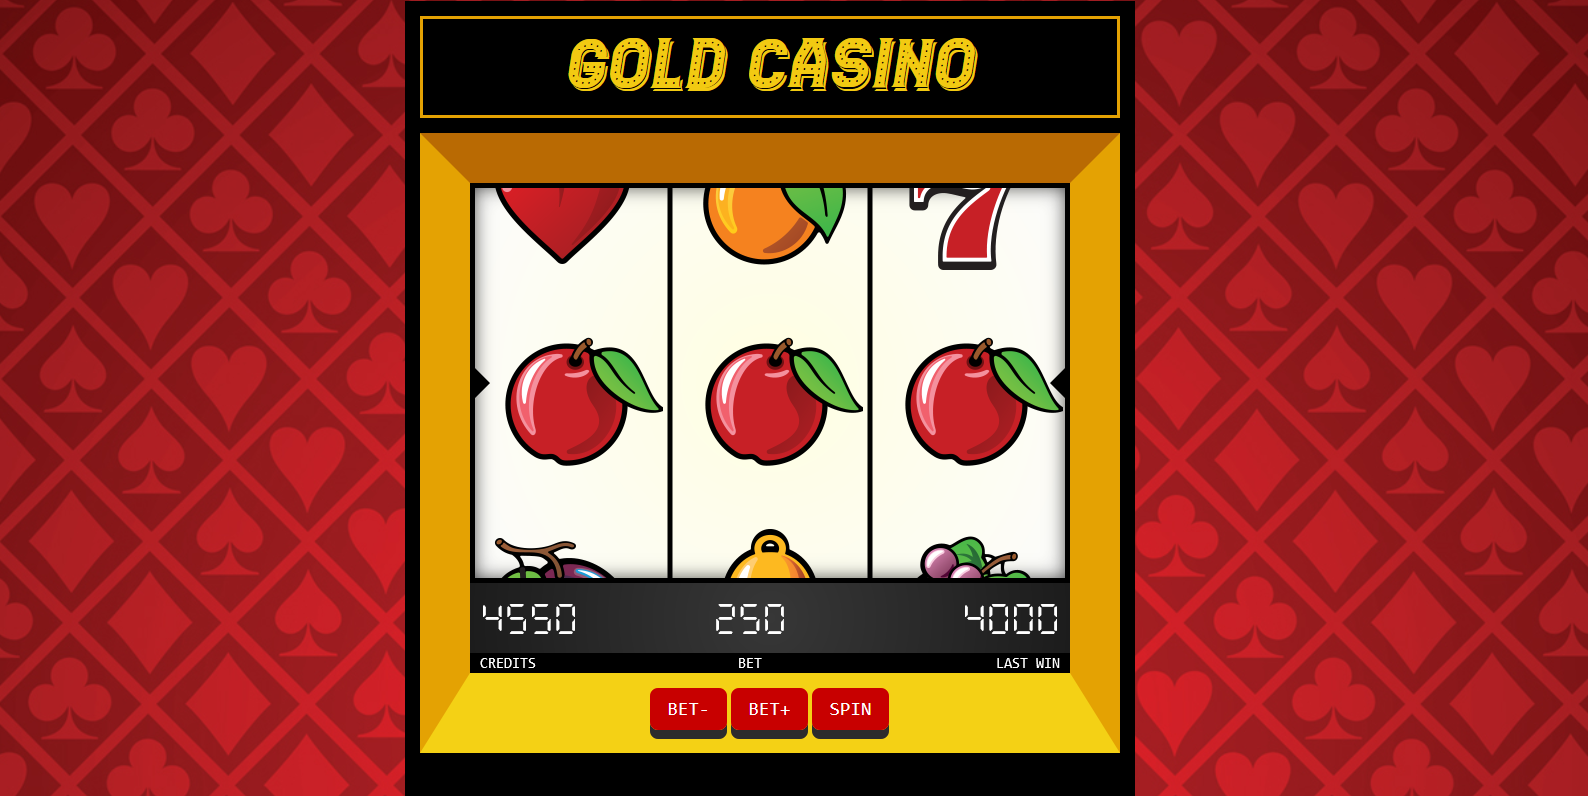
\includegraphics[width=1\columnwidth]{img/screen.PNG}
\caption{Wygląd maszyny losującej} 
\end{figure}

Gracz ma możliwość wylosowania figur spośród 16 różnych elementów (rysunek nr. 2). Biorąc pod uwagę, że koło maszyny losuje po trzy figury, daje nam to kombinację 4096 różnych kombinacji.

\begin{figure}[H]
\centering
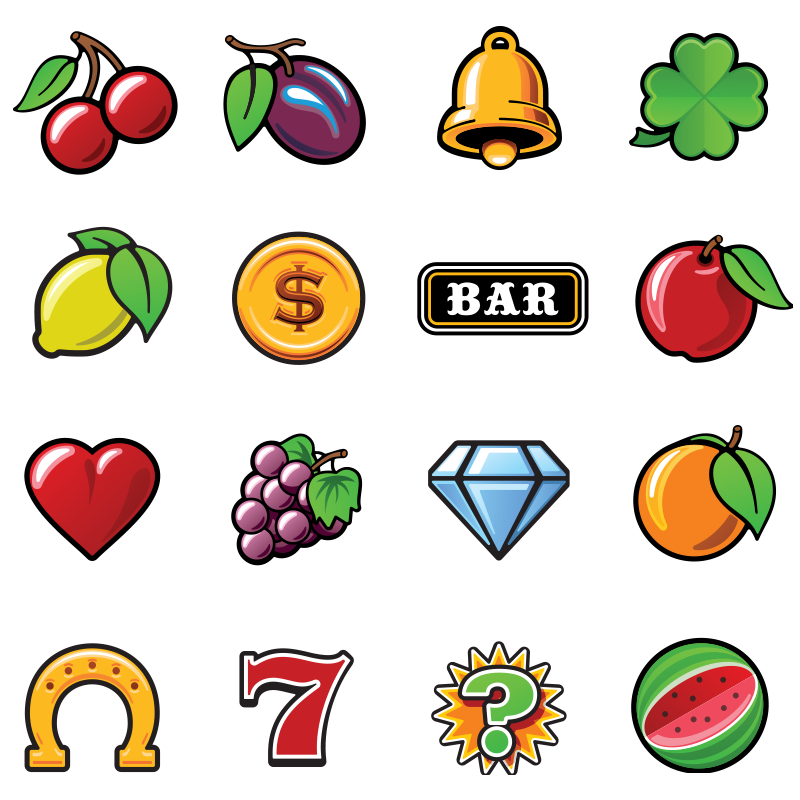
\includegraphics[width=1\columnwidth]{img/ikony.PNG}
\caption{Wszystkie dostępne figury} 
\end{figure}

Gra kończy się w momencie, kiedy nie posiada już kredytów, by ponownie zakręcić kołem. Może on wtedy odświeżyć stronę, by ponownie mieć \verb|$1000| kredytów.

\section{Specyfikacja wewnętrzna}
\subsection{Struktura aplikacji}
Aplikacja składa się tylko z jednego widoku w postaci pliku \verb|index.html|. Pliki kategoryzowane sa na katalogi:
\begin{itemize}
	\item fonts - niestandardowe czcionki zastosowane w projekcie
	\item scripts - logika aplikacji podzielona na wiele plików w celu łatwiejszej rozbudowy
	\item sounds - dźwięki, z których korzysta aplikacja
	\item styles - style .css
	\item images - wszystkie obrazy użyte w aplikacji
\end{itemize}

Wszystkie pliki przechowywane są lokalnie, nie zostały zastosowane żadne zewnętrzne biblioteki dzięki czemu aplikacja będzie działała tak samo online jak i offline.

\subsection{Zasoby dodatkowe}
Aplikacja korzysta z zasobów, które pobrane zostały z internetu, między innymi obrazy figur, zdjęcie tła, wszystkie zastosowane dźwięki oraz niestandardowe czcionki. Adresy do tych zasobów umieszczone zostały na końcu dokumentacji.

\subsection{Uruchomienie aplikacji w środowisku deweloperskim}
Do uruchomienia aplikacji wymagana jest przeglądarka internetowa. W projekcie nie użyto żadnych specjalnych frameworków ani technologii, zatem do edycji wystarczy zwykły notatnik bądź program z podświetlaniem składni. Uruchomienie następuje przez otwarcie w przeglądarce pliku \verb|index.html|.

\subsection{Użyte technologie}
Do wykonania projektu użyłem standardowych technologii webowych:
\begin{itemize}
	\item HTML5
	\item Canvas
	\item JavaScript
	\item CSS
\end{itemize}

\section{Podsumowanie}
\subsection{Testy}
Aplikacja przetestowana została na przeglądarkach takich jak:
\begin{itemize}
	\item Google Chrome
	\item Firefox
	\item Opera
	\item Safari (Mobilne)
	\item Edge
	\item Internet Explorer
\end{itemize}

Wszystkie wyżej wymienione przeglądarki (poza Internet Explorerem) nie wykazywały żadnych problemów w obsłudze aplikacji. Priorytetem podczas tworzenie aplikacji było jej sprawne działanie na wszystkich nowszych i popularniejszych przeglądarkach (do których IE się nie zalicza).

Dodatkowo, projekt został umieszczony na zewnętrznym serwerze w celu przetestowania go online. Adres strony, na której znajduje się projekt: \newline \verb|projects.talar.tech/pwag|

\subsection{Błędy}
Podczas tworzenia aplikacji pojawiały się mniej lub bardziej znaczace błędy, które sukcesywnie były usuwane. Jednym z nich był problem, kiedy aplikacja umieszczona na zewnętrznym serwerze najpierw pobierała skrypty, a na końcu dopiero pobierała obrazy niezbędne do działania aplikacji w związku z czym poczatkowo koło maszyny było puste. Problem rozwiązałem inicjalizując grę dopiero po załadowaniu tagu \verb|<body>|.

\subsection{Możliwość dalszego rozwoju}
Projekt został napisany tak, by zminimalizować trudność jej dalszego rozwoju w związku z czym istnieje perspektywa na jej ulepszanie bądź też połączenie z inną aplikacją (np. z serwerem, który losowałby nagrody i przypisywał do konta użytkownika). Istnieje również możliwość zmiany obrazów figur. Na chwile obecną pobierane są one z jednego pliku .png, który jest ``cięty'' na równe kawałki po 200 pikseli.

\subsection{Wnioski}
Canvas wprowadzony w HTML5 w moim odczuciu jest zbliżony w programowaniu do języka Processing. Programowanie przy użyciu tej technologii wydaje się być całkiem proste, intuicyjne i przyjemne. Mimo tego, część elementów wizualnych realizowałem również przy użyciu html i CSS ponieważ dawało to lepszy efekt.


\newpage
\addcontentsline{toc}{section}{Spis rysunków}
\listoffigures
\newpage


\begin{thebibliography}{9}
\addcontentsline{toc}{section}{Materiały}
\bibitem{canvas}
https://developer.mozilla.org/pl/docs/Web/HTML/Canvas

\bibitem{background}
https://www.deviantart.com/giozaga/art/Casino-Card-Background-Wallpaper-HD-1920x1080-454608180
\bibitem{font-casino}
https://www.dafont.com/casino-2.font
\bibitem{font-digital}
https://www.1001fonts.com/digital-7-font.html
\bibitem{icons}
https://www.vectorstock.com/royalty-free-vector/slot-machine-symbols-set-vector-1067277
\bibitem{sound}
https://youtu.be/UpkC0vMxdDU
\bibitem{sound2}
https://youtu.be/lyZOe9pkZNY
\bibitem{sound3}
https://youtu.be/ZG-VFZ87U7o
\bibitem{sound4}
\verb|https://youtu.be/Sx_LA9OUdVE|


\end{thebibliography}
\end{document}